\chapter{编译和烧录}
\label{ch:compileflash}

本章用一个调试工程，把“填参数”到“固件进板子”的完整链路走一遍。调试工程只关心板子上的
输出：每一路引脚可以单独启用、排序、设参数，固件按顺序逐项执行，跑完最后一项自动回到
第 1 项循环。它不涉及遥控器、底盘与云台，因此最适合在装车之前验证接线、供电、电机转向
和工具链。整个过程分四步：填写参数、静态检查、生成并编译代码、烧录，对应向导左侧的
四个步骤。

\section{用调试工程驱动第一个电机}

\subsection{填写电机参数}

从首页“新建项目”开始，在项目类型中选择“调试”，填写项目名称与保存位置后点击“创建项目”。
向导进入第 1 步“测试序列”，如图~\ref{fig:ch02-tests} 所示。

\begin{figure}[htbp]
  \centering
  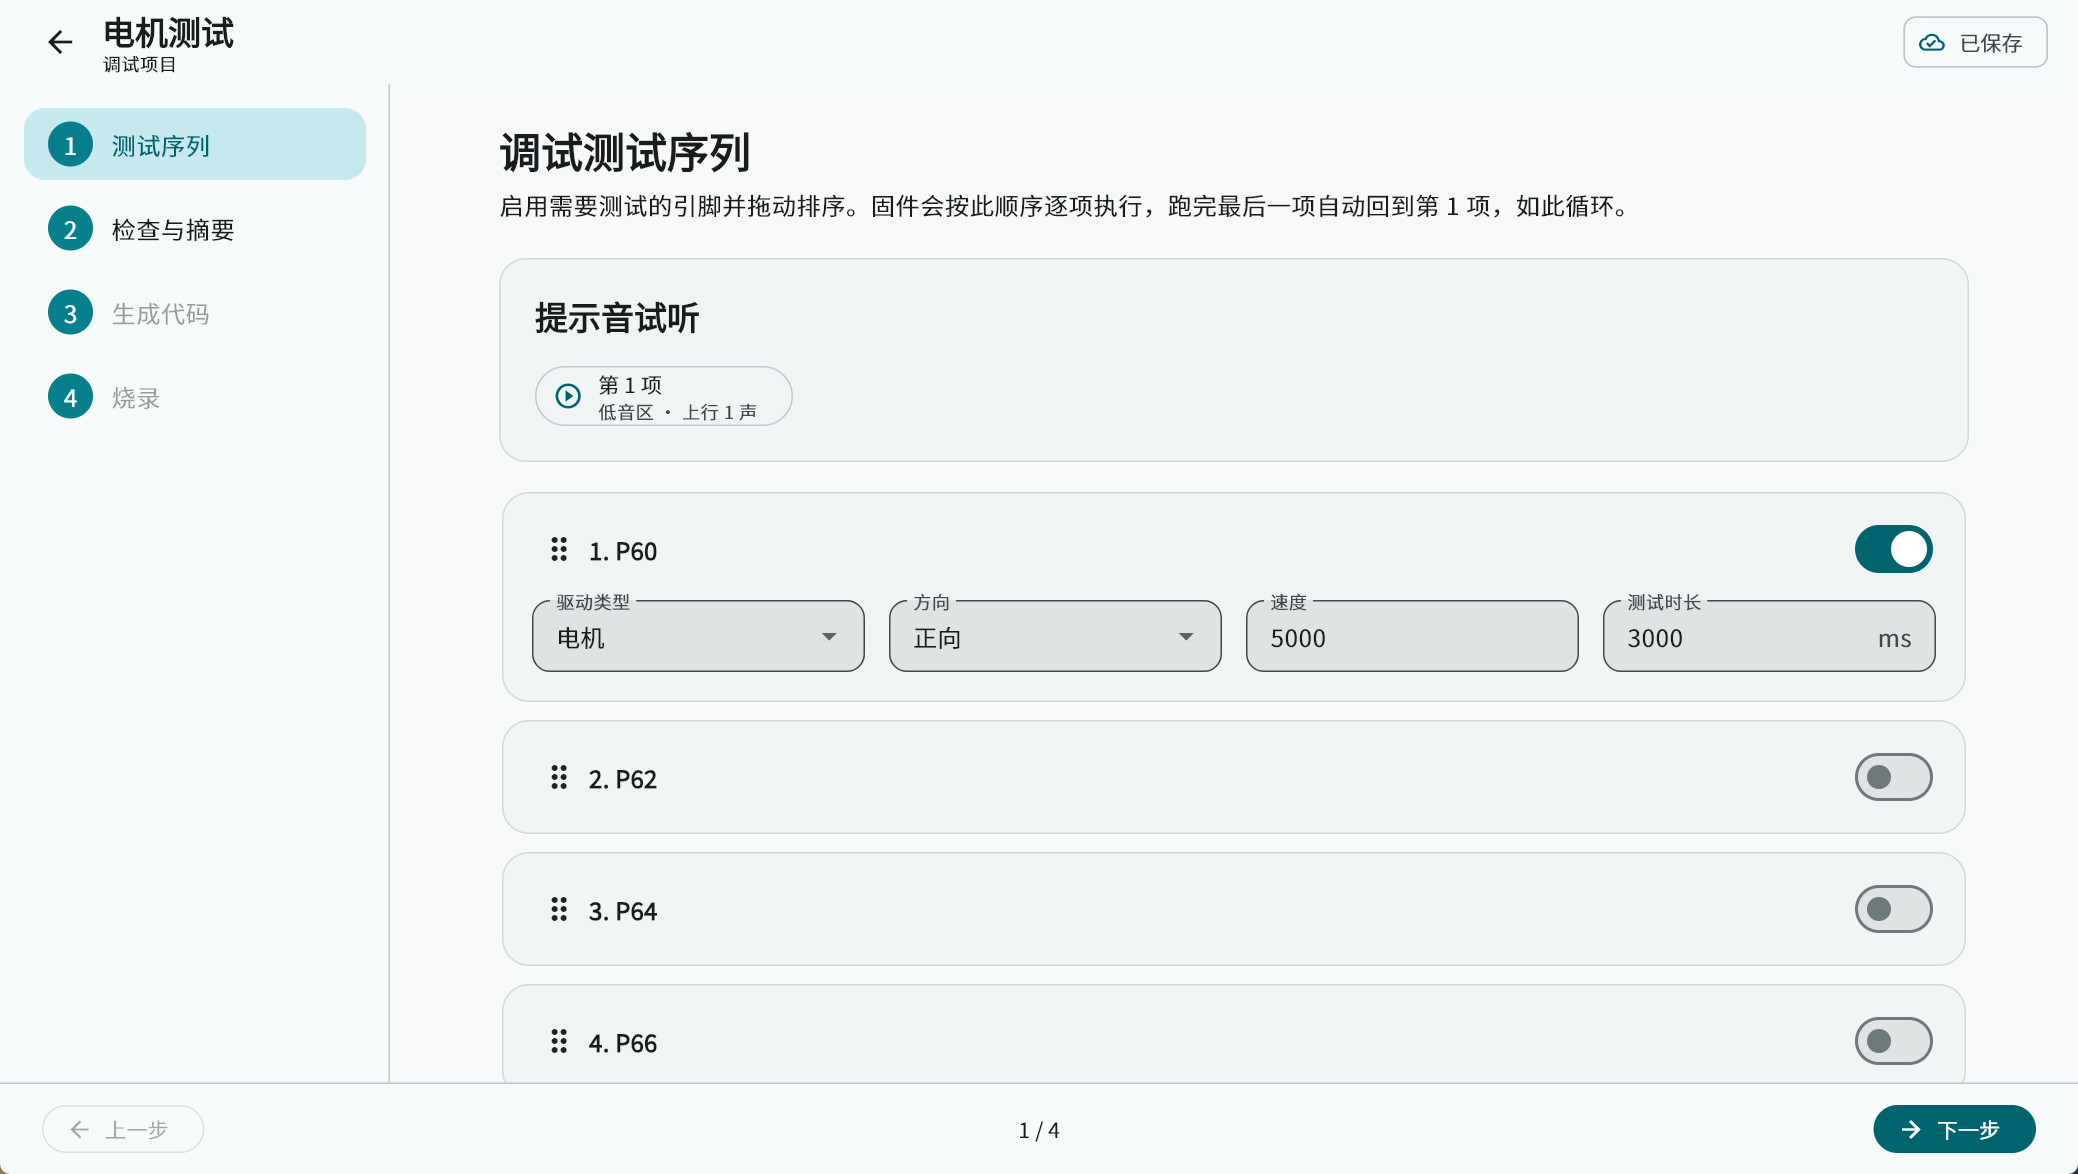
\includegraphics[width=0.92\linewidth]{image/ch02/2-1-tests.png}
  \caption{调试工程的“测试序列”页：启用 P60 并填写电机参数}
  \label{fig:ch02-tests}
\end{figure}

页面列出主控板的十路输出，每一路都有独立开关：打开开关后才会展开参数，关闭的项不会写进
固件。以 P60 为例，打开开关后依次填写：

\begin{itemize}
  \item \textbf{驱动类型}：电机、舵机或摩擦轮。引脚能力不同，下拉框只给出该引脚支持的
        类型；
  \item \textbf{方向}：正向或反向，用来在不改接线的情况下纠正转向；
  \item \textbf{速度}：电机为速度值，舵机为角度，摩擦轮为最大占空比；
  \item \textbf{测试时长}：该项持续的时间，单位为毫秒。
\end{itemize}

示例中 P60 设为“电机 / 正向 / 5000 / 3000 ms”。左侧的拖动手柄可以调整顺序；固件会按
列表顺序逐项执行，跑完最后一项后自动回到第 1 项，如此循环。页面上方的“提示音试听”把
第 $N$ 项对应到上行音型的第 $N$ 个音，装车后即使看不到屏幕，也能凭声音判断当前执行到
哪一项。右上角的“已保存”表示配置已经自动写入项目文件，不需要手动保存。

\subsection{静态检查}

点击“下一步”进入第 2 步“检查与摘要”，如图~\ref{fig:ch02-review} 所示。检查结果分
“错误”与“警告”两类：错误会阻止生成代码，警告只做提示。示例配置只有一项，检查结果为
0 错误、0 警告，页面提示“配置检查通过，可以生成代码”。

\begin{figure}[htbp]
  \centering
  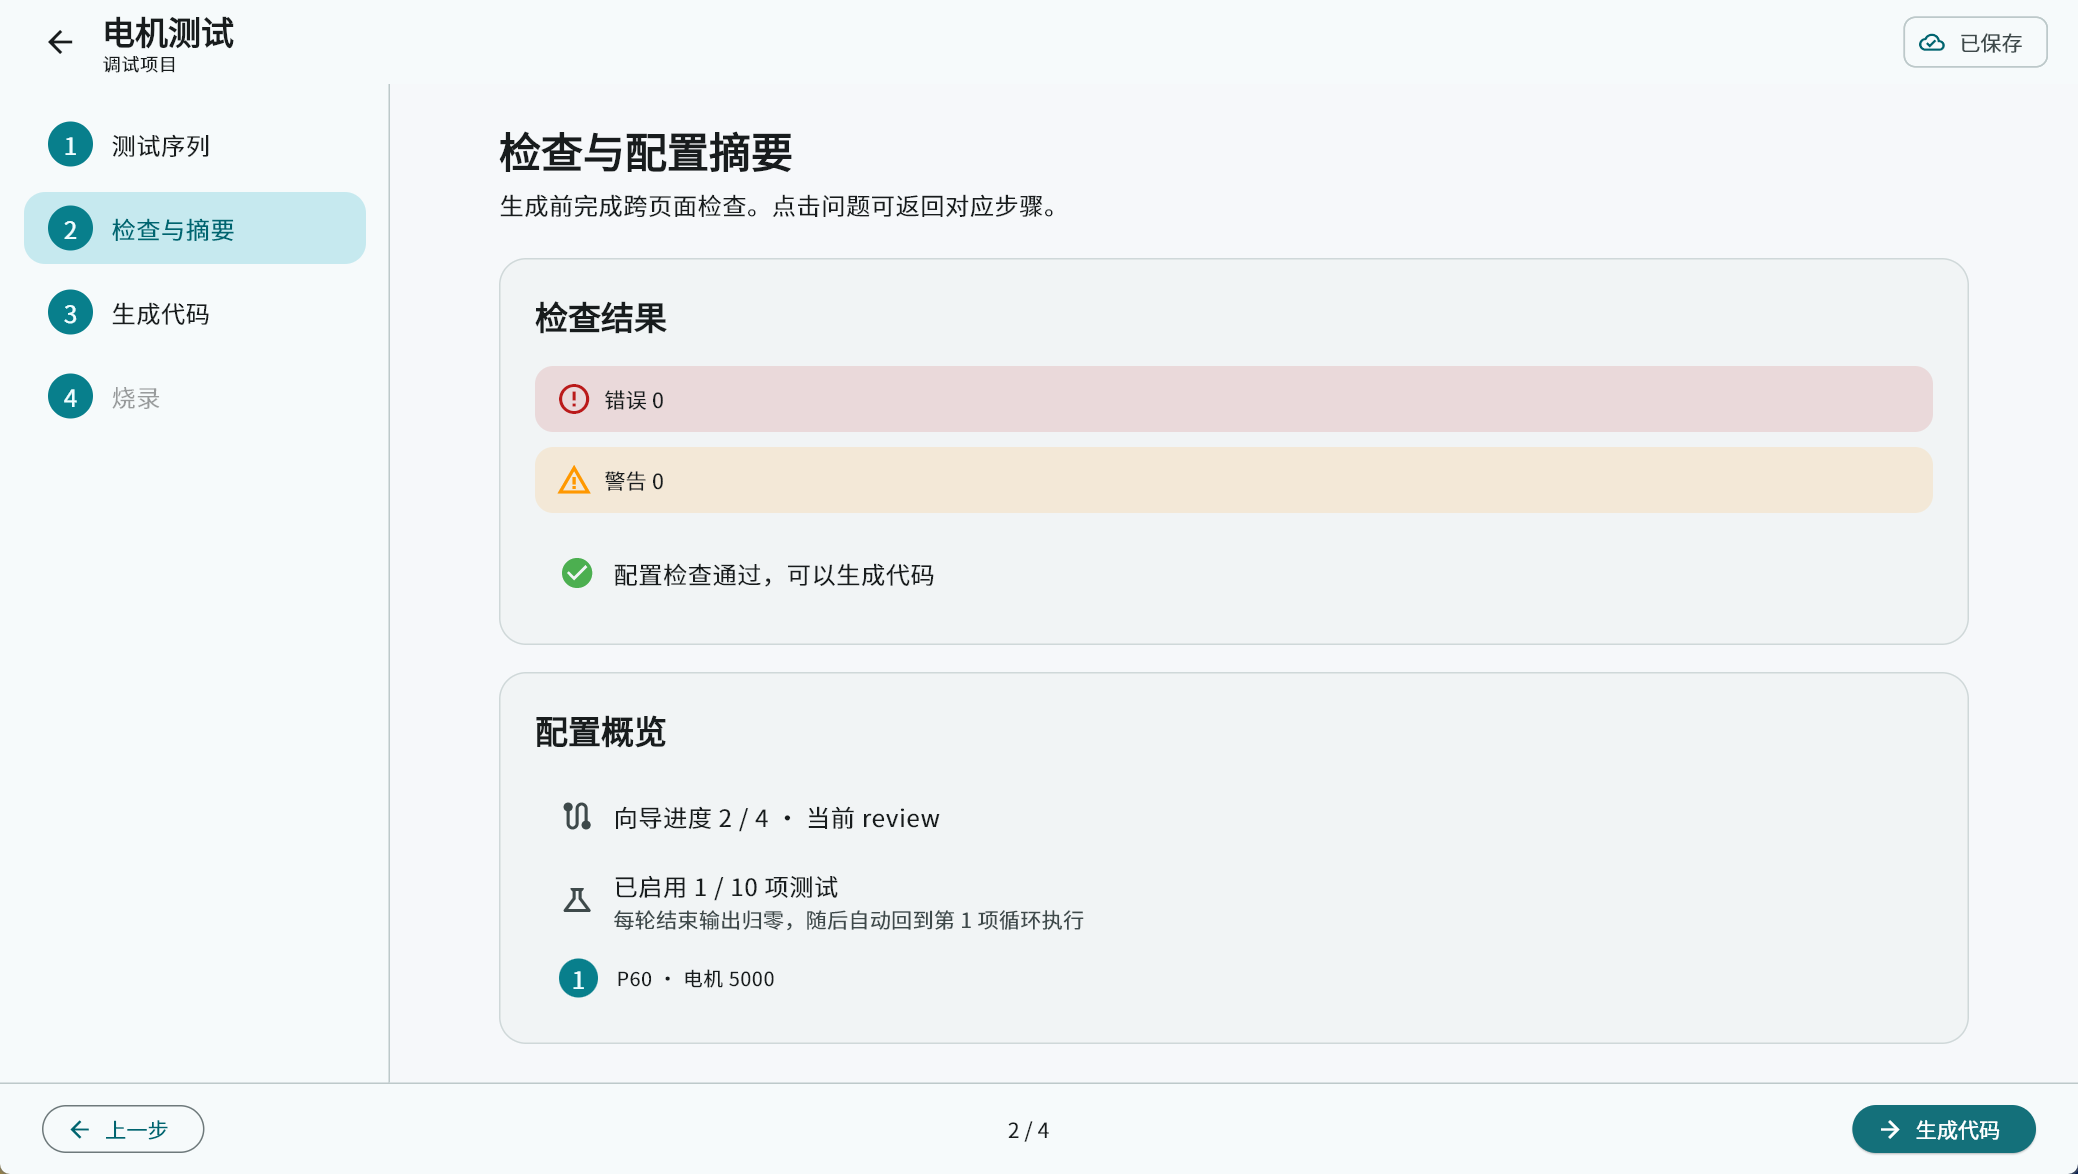
\includegraphics[width=0.92\linewidth]{image/ch02/2-2-review.png}
  \caption{“检查与摘要”页：错误与警告计数均为 0，可以生成代码}
  \label{fig:ch02-review}
\end{figure}

“配置概览”把向导进度、已启用的项数和每一项的摘要列在一起，方便在生成前最后核对一遍。
如果有问题，列表里的每一条都可以点击，直接跳回对应的步骤修改；改完再回到检查页，计数
会随之更新。

\subsection{代码编译}

进入第 3 步“生成代码”，页面默认显示根据当前配置实时生成的 \texttt{main.c}。代码只读，
不会写回项目文件；可以搜索、复制或“另存为”。此时还没有编译——点击右上角的“汇编”，
PIE-Block 才会调用内置的 SDCC C251 工具链做一次完整构建。

\begin{figure}[htbp]
  \centering
  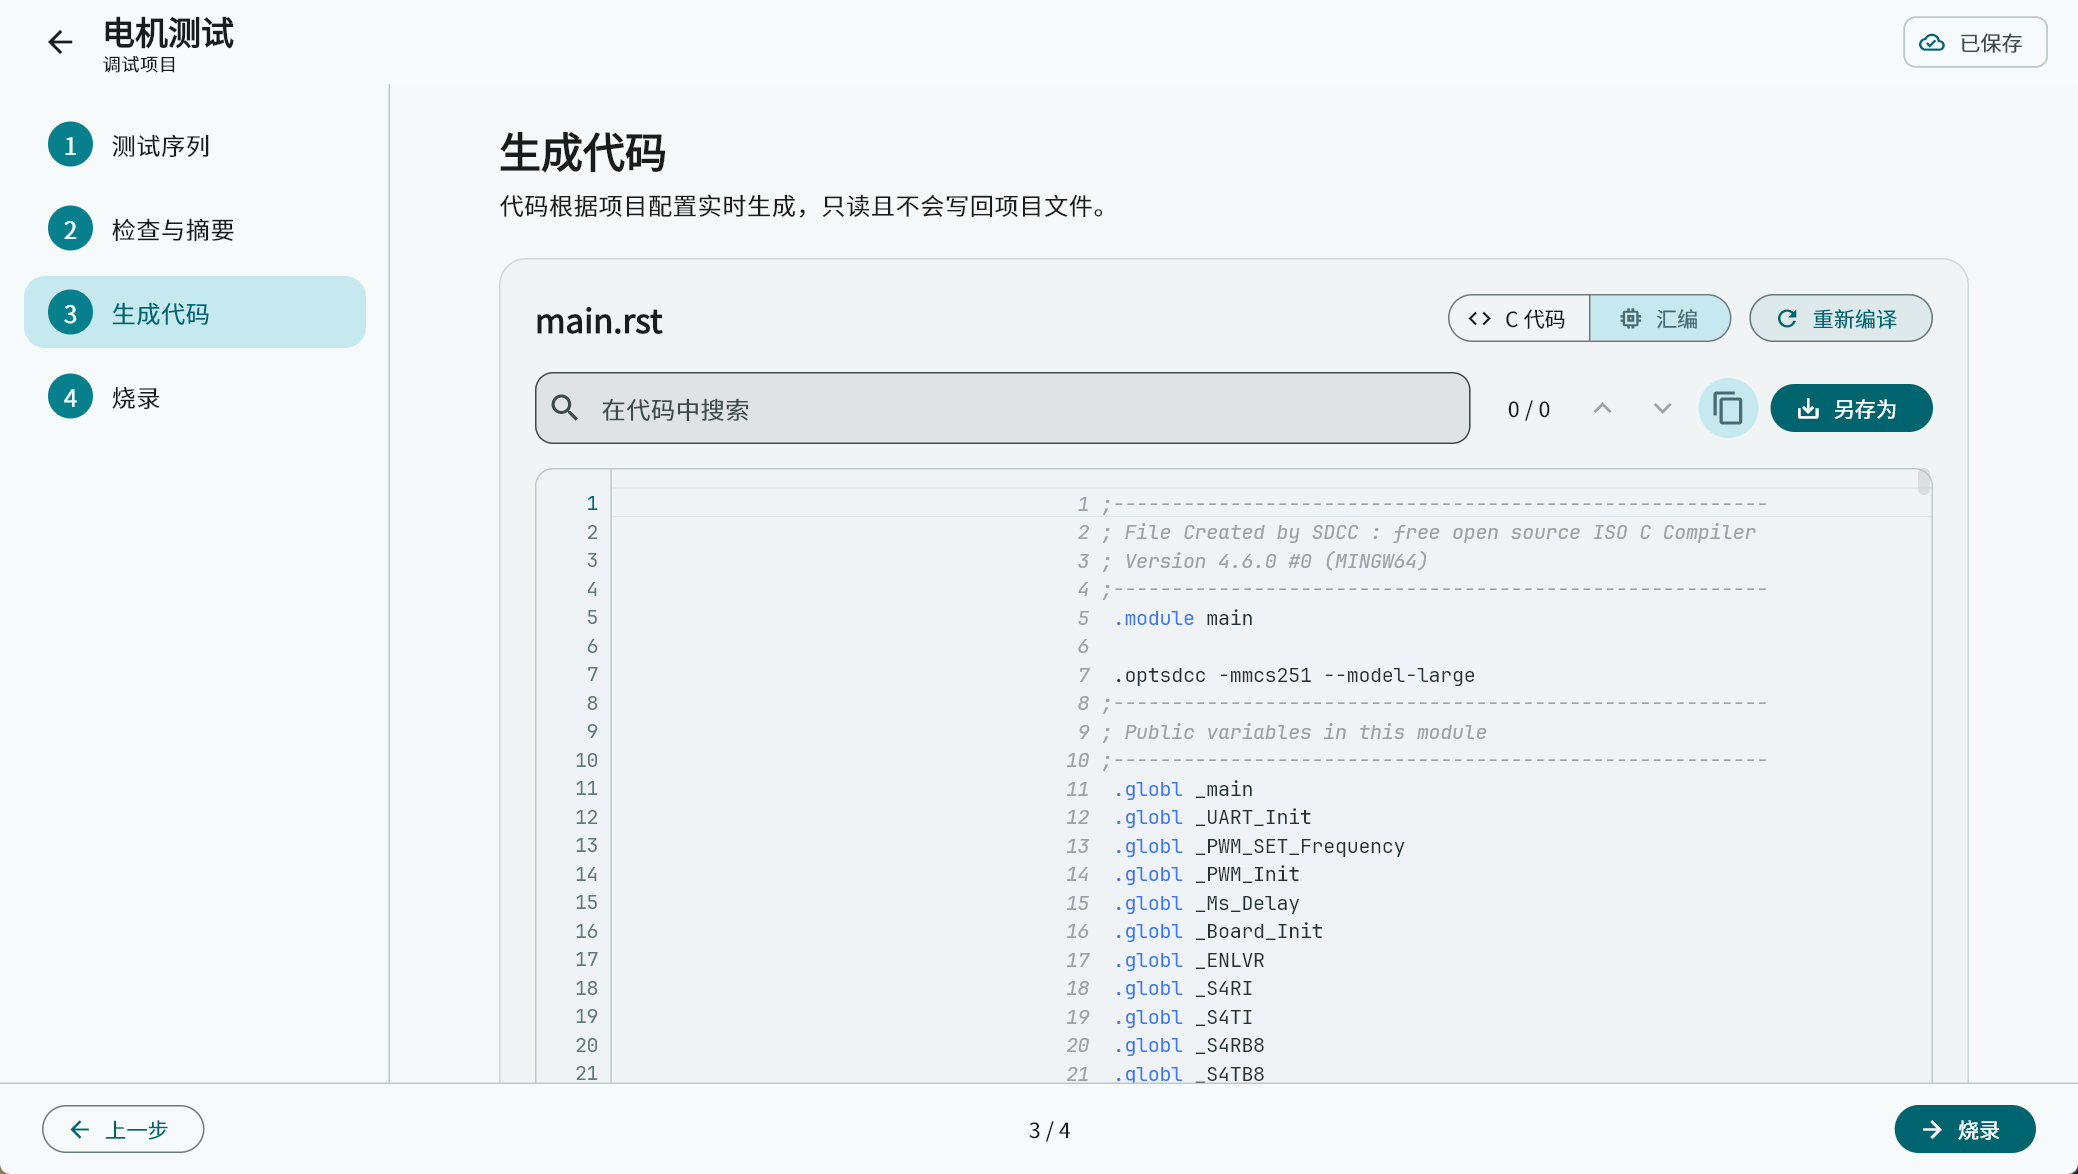
\includegraphics[width=0.92\linewidth]{image/ch02/2-3-listing.png}
  \caption{切到“汇编”后，PIE-Block 调用内置 SDCC 编译并显示 \texttt{main.rst} 列表文件}
  \label{fig:ch02-listing}
\end{figure}

构建完成后，代码区显示链接后的列表文件 \texttt{main.rst}，如图~\ref{fig:ch02-listing}
所示。列表里同时给出地址、机器码、汇编指令和对应的 C 源码位置，可以直接看到一行 C 被
编译成了哪几条指令。文件开头是 SDCC 的版本与编译选项（\texttt{.optsdcc -mmcs251
--model-large}），后面是模块与符号定义。改动配置后源码会变化，再点“重新编译”即可得到
新的列表；构建失败时，占位区会给出失败原因。

\subsection{烧录}

第 4 步“烧录”如图~\ref{fig:ch02-deploy} 所示。页面顶部选择编译器：“内置 SDCC C251”
可完全离线使用，“Keil C251”则调用本机安装的 Keil。示例使用内置工具链，构建产物为
36344 字节，并给出生成时间与警告数。

\begin{figure}[htbp]
  \centering
  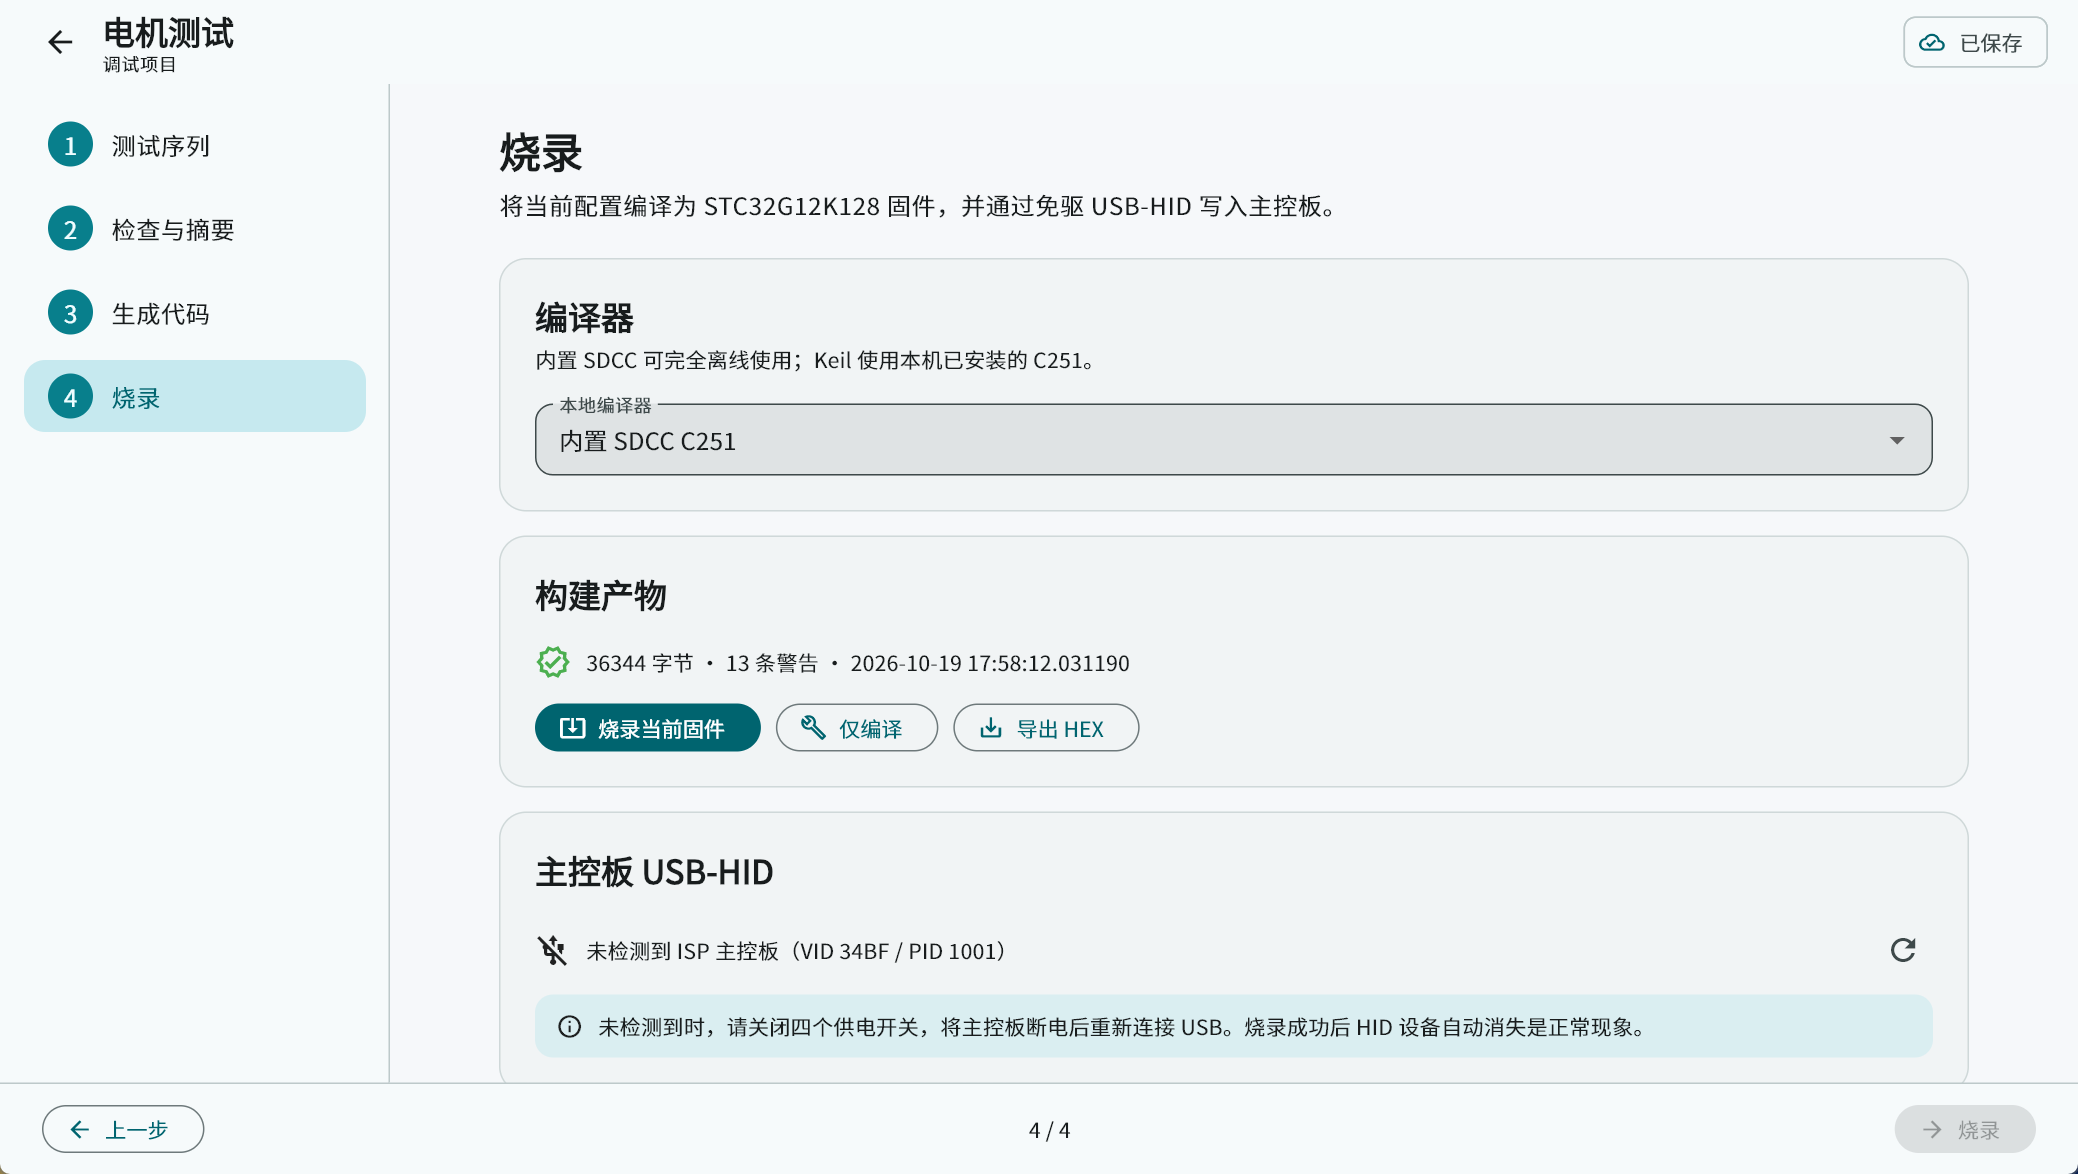
\includegraphics[width=0.92\linewidth]{image/ch02/2-4-deploy.png}
  \caption{“烧录”页：选择编译器、查看构建产物并连接主控板}
  \label{fig:ch02-deploy}
\end{figure}

“构建产物”一栏提供三个操作：“烧录当前固件”“仅编译”和“导出 HEX”。没有主控板时，
可以先用“仅编译”确认配置与工具链没有问题，再把 HEX 交给别的工具。

真正的烧录走 USB-HID：把主控板接到电脑，页面检测到 ISP 设备（VID \texttt{34BF}、
PID \texttt{1001}）后，“烧录当前固件”才可用。若显示“未检测到 ISP 主控板”，按页面
提示关闭四个供电开关、把主控板断电后重新连接 USB；烧录成功后 HID 设备自动消失是正常
现象。烧录过程中的日志与进度会显示在下方，失败时保留原因，便于对照附录~B 排查。
